\chapter{Background}
\label{chap:background}

In the following, first the preliminary information about crowdsourcing concepts 
is summarized, since crowdsourcing is a relatively area of computation. Later,
the related studies and works are examined thoroughly.

\section{Preliminaries}
Crowdsourcing term is first proposed by Jeff Howe~\cite{Howe2006b} in 2006. 
Although there are a long list of terms (collective intelligence, social computing, 
human computation, global brain etc.), in which some of them are new and some 
others are old, the use of term "crowdsourcing" in the academia (demonstrated in 
Figure~\ref{fig:keywordstats}) indicates that research on this domain is promisingly 
increasing.

\begin{figure}[ht]
	\label{fig:keywordstats}
	\centering
	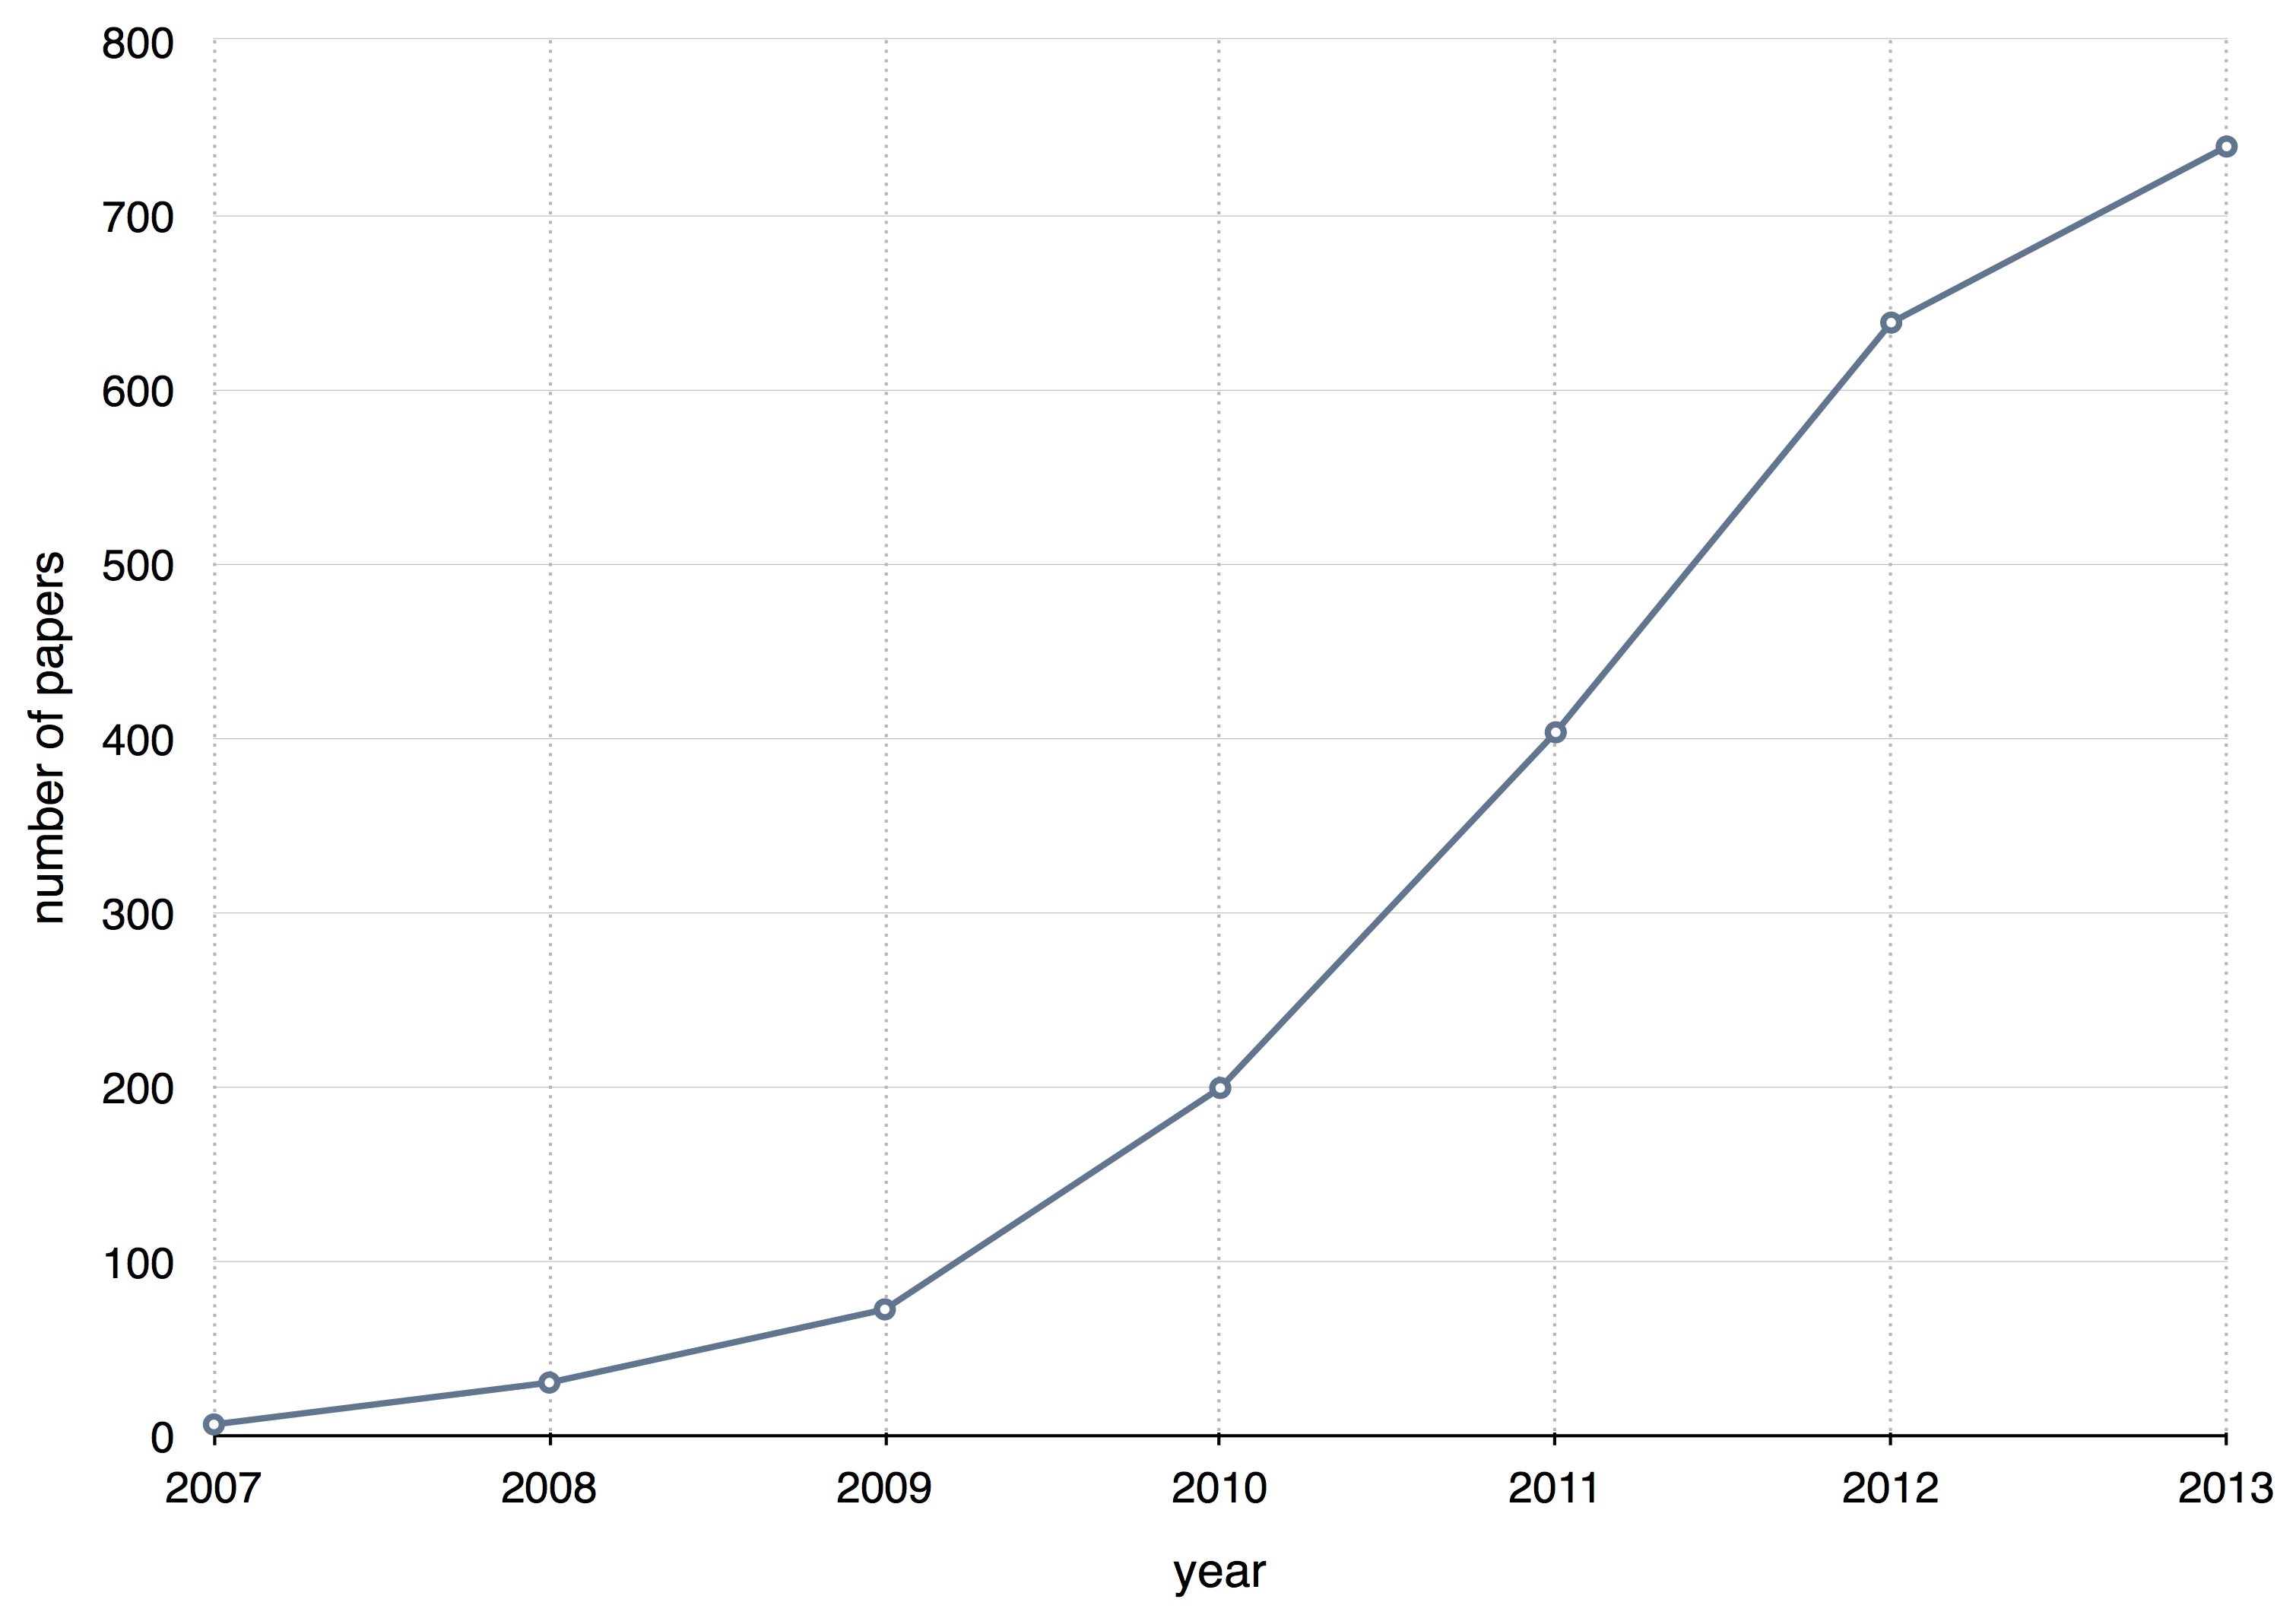
\includegraphics[width=0.85\textwidth]{figures/keyword_statistics.png}
	\caption{The frequency of crowdsourcing keyword in academic papers.}
\end{figure}

The discussion in this section concentrates on Amazon's Mechanical Turk (MTurk).
MTurk is an intermediary platform between employers (known as requesters) 
and employees (workers or turkers) for various-sized and difficulty assignments. 
The platform has become successful for tackling the problems that cannot be 
solved by computers and subject to numerous research studies.

\subsection{Tasks}
Task is a piece of work to be done by the crowd. Terms task, micro-task and job 
are interchangeably used. The term Human Intelligent Task or HIT is commonly 
used as well. A task is often expressed over an HTML form in which there are three 
different input types: single selection (radio buttons), multiple selection (checkboxes) 
and free text (text areas). For single and multiple selection one or more items can be 
selected from a list of possible options. Considering free text types workers are 
supposed to enter a textual response that can be paragraph(s) or sentence(s) 
or number(s).

In addition to the labels attached to input forms, task has a short description 
that provides the instructions and keywords, which will help workers search for 
specific tasks. Further, number of assignments (copies) that requester want completed 
per task can be set. Additional copies of the same task allows parallel processing. 
In that case, the system is supposed to ensure that the parallel workers are unique 
(i.e., no single worker complete the same task more than once).

A task is generally simple requiring small amount of time and expertise to complete. 
In the following, sample tasks from MTurk are presented.

[Sample Tasks Figure Will Come Here]

Tasks can be grouped into task groups. Task groups are for the tasks that share 
similar qualities such as tasks to tag images of nature and people or tasks asking
for translation of a text snippet from a language to another.

\subsubsection{Time}
Often time scale requiring to complete a task ranges from seconds to minutes. 
Nearly 20\% of tasks takes less than 1-hour, and more than half of tasks does not 
take more than 16-hours~\cite{Ipeirotis2010}. Maximum time allotted per 
assignment can be set by requester. 

\subsubsection{Payment}
Compensation or reward for completing tasks range from a single penny to dollars. 
An analysis of MTurk showed that 90\% of tasks pays \$0.10 or less~\cite{Ipeirotis2010}.

\subsubsection{Acceptance}
Once a worker completes and submits an assignment, the requester is notified. 
The requester has an option to either accept or reject the completed assignment. 
Acceptance of an assignment, which indicates the work done is satisfactory, 
makes the worker who completed it get paid, on the other hand rejection withholds 
payment for which the reasoning may or may not be provided by the requester. 
Another option is automatic approval, which is the case when requester does not 
review work after a some time that can be set by the requester.

\subsubsection{Expiration}
Tasks have a lifetime limit that decides the amount of time that a particular task 
remains in the listings. Lifetime can be set by requester. After a task reaches 
end of its lifetime, it is automatically pulled from the listings.

Another type of expiration can happen while a worker is operating on an assignment. 
When workers accept an assignment, the assignment is reserved for them making 
no other worker to accept it. The reservation is for particular piece of work 
(in this case assignment) and time-limited. If worker does not submit the completed 
assignment in allotted time, then reservation is cancelled and assignment is 
made available for others again.

\subsection{Requesters}
Requesters are the employers who post tasks, obtain results and pay workers. 
Requesters are expected to design tasks with all the details (description, instructions, 
question types, payment, expiration settings etc.) After completed assignments 
are submitted, requesters can review them by accepting or rejecting, 
and collect the completed work. 

These operations can be done via user interface or application programming 
interface (API) if there is one. 

\subsection{Workers}
Workers are the online users or someone from the crowd who work on and 
complete assignments in exchange for a small payment. On some platforms 
(currently not available on MTurk), detailed information about workers are gathered 
and kept in a database. This information can be later utilized by requesters while 
associating specific constraints to the assignments such as limiting age to some 
range for a specific task. 

\subsection{Quality Control}
Quality control is challenge for crowdsourcing platforms, since low quality work 
is common. It is shown that low quality submissions can compromise up to one third 
of all submissions~\cite{Bernstein2010}. As a result, researchers have started to 
investigate several ways of detecting and correcting for low quality work.

Visualization of workflow is one of the methods employed for which directed graphs 
are used to show the organization of crowdsourcing tasks, allowing endusers 
to better understand the problem and proposed solution design~\cite{Kulkarni2012, Kittur2012}.

Application of programming paradigms is another approach taken by 
researchers. MapReduce~\cite{Kittur2011, Ahmad2011}, 
Divide-and-Conquer~\cite{Kulkarni2012}, 
Iterative~\cite{Little2009}, 
Workflow ~\cite{Kokciyan2012} are some of these approaches taken for 
organizing and managing complex workflows. Although these paradigms 
fit perfectly some problems, there are other problems not suited well to those.

Inserting 'gold standard' questions into an assignment with which workers 
who answer them incorrectly can be filtered out or given feedback~\cite{Burch2009}. 
However, writing validation questions create extra burden to requesters and 
may not be applied to all types of tasks.

Majority voting to identify good submissions is proposed as another 
option~\cite{Burch2009, Bernstein2010}, but this technique can be affected 
by majority (especially when the possible options are constrained) or failed in 
situations where there are no answers in common such as creative or generative 
work~\cite{Rzeszotarski2012}.

Systems (including MTurk) often do not apply any of these quality control approaches, 
but provide other ways to achieve good workers and discourage bad ones. 
Currently each worker on MTurk has an acceptance rate that is updated after 
requester's review on completed assignments. However, this feature does not 
differentiate one type of task from the other in terms of effect on acceptance rates 
and that makes it a limited utility. A worker who is skilled in audio transcription would 
probably have high accuracy rating in related tasks. However, there is no way to 
reason that this worker can also perform English-to-Turkish translation tasks. 
Even worse is that workers who pick and complete easy tasks would probably 
have higher accuracy rates than the ones who choose to perform tasks that 
require time and expertise~\cite{Barowy2012}.

Requesters can utilize acceptance rates by assigning a low limit of them to 
assignments, which allow only workers with acceptance rates above-limit 
to accept assignments.



\section{Related Work}
In response to the challenges of crowdsourcing a number of attempts have been made 
by the researchers. In the following, the studies that related to this work are listed, 
described and examined in detail. The studies that try to address the challenges of 
crowdsourcing and proposing new way of creating crowdsourcing workflows are
considered as related. Otherwise, the related work list would be too long, 
since many views Wikipedia and Linux as crowdsourcing systems.



\subsection{Crowdsourcing Platforms}
\subsubsection{Jabberwocky}
Jabberwocky~\cite{Ahmad2011} is a social computing stack consists of three 
main components: Dormouse, ManReduce, and Dog. Dormouse is created to 
enable cross-platform human and machine resource management. It acts like a 
"virtual machine" layer in the computing stack, consisting of low-level software 
libraries that interact with people and computers. ManReduce is a parallel 
programming framework for human and machine computation working on top 
of Dormouse. ManReduce is inspired by MapReduce~\cite{Dean2008} that is 
basically mapping problem into a set of small chunks of work, and then reducing 
them on an output that aggregate the responses or solutions. Dog is a high-level 
programming language on top of ManReduce. The language is formed by a small 
set of primitives for requesting computational work from people of machines. 

Jabberwocky is limited in several ways. The computing stack is a command-line 
tool supported by restricted built-in libraries and can only be run on Dormouse server. 
The high-level language, Dog, seems simple, clear and expressive, but still there is 
still a learning curve based on the fact that not all crowdsourcing requesters are 
developers. This is the issue for the command-line tool as well.

Another important limitation is lack of progress idiom within the system. 
Jabberwocky receives script definitions (deployment to Dormouse server), 
a process starts. Once all of them are completed, the output is written to a destination 
file and process terminates. In that respect, there is no way that end user can 
observe the current state of problem-solving.

Even if this work aims at solving general-purpose and real-world problems, 
it is mentioned that real-time and single-worker sequential applications are not 
well-suited. Despite MapReduce paradigm is simple and many social computing 
problems fit naturally to this paradigm, it is obvious that only some set of problems are 
appropriate to be solved using such a paradigm or system, which is another limitation. 

However, Jabberwocky's notion of real identity and social structure, 
which would allow end users to define person-level constraints, is noteworthy.

%Human: Yes
%Machine: Yes
%Heterogeneity: Yes
%Concept: MapReduce
%User-interface: No
%Progress: No
%Programming: Yes


\subsubsection{WeFlow}
WeFlow~\cite{Kokciyan2012} is a collaborative application specification, 
application generator and execution engine proposed in a master thesis~\cite{Kokciyan}. 
A framework is introduced to create and run collaboration-based applications. 
That framework allows end users to decompose problem into tasks, 
describe the computation resources, define the control and data flow.

A task consists of input(s), instruction describing the expected action from user 
and output(s). Task can be a type of basic (the most simple, atomic work definition), 
conditional (execution based on a condition), repetition (recurring execution based 
on a conditional), doall (groups of tasks executed in parallel) or collective 
(multiple times execution). The framework is definitely restricted by 
these predefined task definitions.

Besides task specification, end user should designate the control flow and 
data flow. Control flow determines the order of tasks to-be-executed. 
On the other hand, data flow is defined to map data between and/or within tasks. 
All these specifications are done via XML. Despite the fact that the framework 
is mentioned to require no programming skills and XML is widely used format 
for representing arbitrary data structures, there is a learning process of 
WeFlow specifications not to mention the lack of development 
and debugging environments.

WeFlow differentiates human workers from each other depending on a 
role definition. Participants are linked to some role. Likewise a task is associated 
with a role. Although the whole role definition would allow end user handle access 
control by describing permission-like roles, it does not discriminate human 
performers based on their characteristics such as age, gender, interest, expertise etc.

%Human: Yes
%Machine: Yes
%Heterogeneity: Partially
%Concept: Workflow
%User-interface: No
%Progress: No
%Programming: No

\subsubsection{TurKit}
TurKit~\cite{Little2009} is a toolkit for deploying iterative tasks to MTurk. 
Toolkit is based on a model that concentrate on iterative work in which series of 
individuals work on tasks that are previously completed by others. Although 
creators of TurKit apply several nontrivial problems (image description, 
brainstorming, writing tasks, sorting etc.) to the iterative model, this work 
majorly restricted by the iterative paradigm that toolkit operates on. The complex 
and sophisticated problems that are expected to be addressed by crowdsourcing 
systems do not often correspond to iterative model.

TurKit API is defined to help writing iterative MTurk tasks. However, TurKit expects 
end user to be a programmer and create HTML pages for tasks, and write 
Javascript files using API. In fact, end user is responsible for testing and making 
sure that the pages with TurKit functionality interact properly with MTurk. 
This just reveals another major limitation of TurKit on it's usefulness.

However, the toolkit have some notion of fault tolerance preventing wasted 
money or time due to bugs and system crashes. Toolkit stores information about 
the trace of a program's execution. This trace is used whenever program crashes 
and to put the program back into it's previous state. Thus, toolkit does not 
re-execute the whole program, but the sections where they are left unfinished.

%Human: Yes
%Machine: No
%Heterogeneity: No
%Concept: Iterative
%User-interface: No
%Progress: No
%Programming: Yes

\subsubsection{CrowdLang}
CrowdLang~\cite{Minder2011} is a general-purpose framework and a concept of 
an executable, model-based programming language for workflow definition. The 
framework is developed based on the assumption that a complex problem is 
characterized by defining the problem, decomposing the problem into subproblems, 
planning subproblems, executing the plan and aggregating the solutions of subproblems.

CrowdLang programming language is based on a small set of operators: 
Divide-and-Conquer, Aggregate, Multiply, Merge, Router and Reduce 
(functionality of operators can be understood by their names). These operators 
are combined together to solve complex problems by routing, distributing and 
task decomposition. In addition, different types of genes are defined to address 
various participation patterns.

This work introduces a good and novel concept for general-purpose crowdsourcing 
that is suitable to most problems. The framework is not bounded to some other 
programming paradigm or limited to only one aspect of crowdsourcing. It rather 
supports complex coordination mechanisms. In this respect, translation, which is a 
sophisticated and difficult problem for crowdsourcing, is attempted in ~\cite{Minder2012} 
and the results (translation of 15 different articles in less an hour) are promising.

%Human: Yes
%Machine: Yes
%Heterogeneity: No
%Concept: None
%User-interface: No
%Progress: No 
%Programming: Yes

\subsubsection{AutoMan}
AutoMan~\cite{Barowy2012} is described to be a fully automatic crowd programming s
ystem. It is a programming system integrating human and computer computation. 
On top of AutoMan system, a domain specific programming language is defined. 
It is implemented as embedded domain-specific language for Scala.

The system's whole crowdsourcing concept is based on Question objects. 
Question can be type of radio-button, checkbox and restricted free-text. The human 
computation aspect of system only corresponds to the answers given by individuals. 
Further, system provides no mechanism to design complex problems through a 
set of subproblems or tasks. This makes system no advantageous to the 
existing systems depending on simple tasks.

In fact, end users are supposed to write programs in AutoMan DSL and provide 
them to the system. Considering the examples in the paper, the learning curve 
for this language can be expected to be high, because it requires knowledge 
of Scala language (comparing with Dog introduced in~\cite{Ahmad2011}).

However, scheduling, pricing and quality control mechanisms are significant 
components of AutoMan. The runtime system has a scheduling component that 
periodically checks the current situation of the results, and reprices and restarts 
human tasks as necessary. By making this, system tries to achieve the predefined 
confidence level (by end user) while staying under budget.

%Human: Yes
%Machine: Yes
%Heterogeneity: No
%Concept: None
%User-interface: No
%Progress: No
%Programming: Yes

\subsubsection{Turkomatic}
Turkomatic~\cite{Kulkarni2012} is a tool that recruits workers for planning and 
solving complex tasks. The system executes price-divide-solve approach by 
asking workers to divide complex steps into simpler ones until they are at a simple 
level, then to solve them. The approach simply uses divide-and-conquer strategy, 
but the division is done by the crowd different from other crowdsourcing systems.

The system has a set of pre-structured task templates. End users can produce 
workflows by combining templates together without implementing any software 
or designing intermediate tasks. The price-divide-solve approach is expected 
to produce a directed, acyclic task graph in which nodes represent subtasks and 
links describe task dependencies. The user interface visualizes the task graph 
and enables endusers delete or modify them in real-time.

The system is significant by demonstrating complex problems through acyclic 
task graphs. The graphs are not just shown to the endusers, but also implemented 
in a way that enables real-time modification. However, initial workflow design 
is left to workers by a single instruction (a few sentences) telling what the enduser 
achieve in the end. This approach is limited by the efficiency of instruction and 
understanding of workers, and reportedly not really successful. It is mentioned 
that for complex work manual intervention and editing of workflow is effective.

Currently the system's crowd planned workflows are not guaranteed to be 
context free. This restricts the set of problems that the system can tackle, 
but still this study presents promising results by demonstrating and managing 
complex problems through acyclic graphs.

%Human: Yes
%Machine: No
%Heterogeneity: No
%Concept: Divide-and-Conquer
%User-interface: Yes
%Progress: No
%Programming: No

\subsubsection{CrowdForge}
CrowdForge~\cite{Kittur2011} is a general-purpose framework and toolkit for 
accomplishing complex and interdependent tasks using micro-task markets. 
The framework is built on MapReduce~\cite{Dean2008} approach, which first breaks 
down a complex problem into a sequence of subproblems, and combines the results 
later. A similar approach is taken for the design of ManReduce in Jabberwocky 
stack~\cite{Ahmad2011}.

Although CrowdForge approach is designed to fulfill complex problems, it is still limited 
to the capabilities of MapReduce approach. Some problems may not be addressed 
by this approach such as the case for tasks that cannot be really decomposed. 
Another case would be when subtasks are not independent, but the state 
or result of one is important to complete the other. All these exemplifies the 
limitations of the approach taken from distributed computing field and 
expected to fit well in crowdsourcing.

Additionally system has no support for iteration or recursion. It requires the 
end user (task designer) to specify each stage (partition, map, reduce) in the task flow.

%Human: Yes
%Machine: No
%Heterogeneity: No
%Concept: MapReduce
%User-interface: Yes
%Progress: No
%Programming: No

\subsubsection{CrowdWeaver}
CrowdWeaver~\cite{Kittur2012} is a system to visually manage crowd work. 
This system comes forward among various other works with it's visual representation 
abilities. High-level representation of a workflow makes it easier for end user to grasp, 
design and develop crowdsourcing programs.

The system has a predefined set of task templates. Workflows are created by 
creating tasks and linking them with each other in various ways. Branching and 
combining multiple data flows are supported and that makes design of complex 
problems possible. 

Besides visualization, CrowdWeaver has a notion of tracking and notification. 
The task progress component monitors the current state and depicts the current state
via graphs. Along with notification component, users can be notified about the 
progress based on the predefined conditions (specified by users). Further, 
it is possible to stop a task and make changes on existing branch in real-time. 

Despite CrowdWeaver demonstrates a system that can be easily utilized by users 
with no programming background, the system is currently limited by predefined set 
of templates. In fact, it's visual abilities are restricted by only showing the workflow, 
but not enabling users make changes on it directly.

%Human: Yes
%Machine: Yes
%Heterogeneity: No
%Concept: Dataflow
%User-interface: Yes
%Progress: Yes
%Programming: No


\begin{sidewaystable}
\label{tab:comparison}
%\bigskip
%\centering
  \begin{tabular}{| l | c | c | c | c | c | c | c | c | }
  \hline
  Feature & Jabberwocky & WeFlow & TurKit & CrowdLang & AutoMan & Turkomatic & CrowdForge & CrowdWeaver \\ \hline
  Concept & MapReduce & Workflow & Iterative & N/A & N/A & Divide-and-Conquer & MapReduce & Data Flow \\ \hline
  Human components & \CIRCLE & \CIRCLE & \CIRCLE & \CIRCLE & \CIRCLE & \CIRCLE & \CIRCLE & \CIRCLE \\ \hline
  Software components & \CIRCLE & \CIRCLE & \Circle & \CIRCLE & \CIRCLE & \Circle & \Circle & \CIRCLE \\ \hline
  Requires programming & \CIRCLE & \Circle & \CIRCLE & \CIRCLE & \CIRCLE & \Circle & \Circle & \Circle \\ \hline
  Heterogeneity & \CIRCLE & \LEFTcircle & \Circle & \Circle & \Circle & \Circle & \Circle & \Circle \\ \hline
  User Interface & \Circle & \Circle & \Circle & \Circle & \Circle & \CIRCLE & \CIRCLE & \CIRCLE \\ \hline
  Progress & \Circle & \Circle & \Circle & \Circle & \Circle & \Circle & \Circle & \CIRCLE \\ \hline
  %\\ \\ \\
  %\multicolumn{9}{l}{\CIRCLE: Yes, \LEFTcircle: Partially, \Circle: No} \\
  \end{tabular}
  \vspace{3 mm}
  \caption*{
  	\begin{tabular*}{1\textwidth}{l l}
		\CIRCLE: & Yes \\
		\LEFTcircle: & Partially \\
		\Circle: & No \\
	\end{tabular*}
  }
  \caption{Comparison of related works}
\end{sidewaystable}

\newpage

\subsection{Other Studies}
\subsubsection{Soylent}
Soylent~\cite{Bernstein2010} is a word processing interface enabling Microsoft Word 
users to employ MTurk workers to shorten, proofread and edit parts of their 
documents on demand. The system is developed with respect to the 
Find-Fix-Verify pattern that is introduced in the same study.

The pattern approaches complex tasks (focused on text editing) by splitting them 
into a series of generation and review stages. Rather than asking a single worker 
to read and edit an entire section, the pattern first recruits a set of workers to 
find areas of improvements. Then, another set of workers review the candidate 
areas and filter out incorrect ones. Finally, in the verify stage workers perform 
quality control on previous submissions. Throughout the process the pattern 
utilizes independent agreement and voting.

Both the system and the pattern concentrates on a small set of use cases of 
crowdsourcing. The system can only be employed by Microsoft Word users 
for editing text. The pattern is limited to the problems where decomposition 
into subproblems is possible.

\subsubsection{Qurk}
Qurk~\cite{Marcus2011, Marcus2011b} is query processing system that 
automatically translates queries into tasks to-be-completed by humans. The system 
has domain-specific language to express tasks. A UDF-like approach is taken 
by integrating SQL with MTurk expressions.

The approach is concentrated on a MTurk-aware database system rather than 
a general-purpose crowdsourcing mechanism. Thus, the set of tasks that can be 
introduced via the system is limited by associated database concepts such as 
joining, sorting etc. Although generative tasks for which workers give unconstrained 
input are made available, still processing is done on input data obtained from the 
underlying database system. However, this study provides an important example 
by employing people in a database system for managing various queries.

\subsubsection{Mobi}
Mobi~\cite{Zhang2012} is a system to crowdsource itinerary plans. The system 
illustrates a use case of crowdware paradigm. The paradigm focuses on tasks 
with global requirements and provides a single workspace in which a crowd of 
individuals contribute opportunistically to the global solution based on their knowledge 
and expertise. Itinerary planning is taken as a case study and implemented 
in Mobi system through a single interface.

In the system and paradigm, the problem definition is limited to the tasks 
with global constraints. This is a clear example of a study that concentrates 
on only one aspect of crowdsourcing. However, the study provides insights 
on the effectiveness of using unified solution context for workers or directing 
crowd's submissions through a structured guide or benefits of iterative refinements.

\subsubsection{CrowdSpace}
CrowdSpace~\cite{Rzeszotarski2012} is a system that supports the evaluation 
of complex crowd work by combining information about worker results through 
visualization. This system focuses on exploration and assessment of worker 
performance and behavior rather than providing ways to manage complex workflows.

The system presents a unified user interface with four components: a scatter plot 
of aggregate behavioral features (time spent on the task, number of keys pressed 
while processing the task etc.), distribution of each behavioral features, 
traces of worker/output pairs and overall worker behavior based on their answers.

Low quality work is common in crowdsourcing. However, this system provides 
great insights by combining worker behavior with their submissions, and enabling 
end users to identify the behavior of workers who have good or bad outputs. 
Although this approach is limited by several aspects such as being only applicable to 
pages in which Javascript can be inserted or assuming that worker does all the processing 
on the page etc, the quality control approach taken in the study can be used to 
better understand and address the nature of the crowd.

\subsubsection{Human Architecture}
Human Architecture~\cite{Dorn2012} is an adaptation mechanism to the changing 
requirements of the various type collaborations. Unlike other studies, this work focuses 
on collaboration problem from the architectural perspective. An architecture description 
language is proposed to describe collaboration dynamics. Considering software architecture 
human components and collaboration connectors are introduced to demonstrate 
coordination dependencies. 

However, the proposed human architecture approach is too architecture focused and 
highly complex. The collaboration of individuals is narrowed down to component 
and connectors, but in the context of complex problems collaboration is dynamically 
changing and highly interactive due to the data items that are output from one 
and input to the other. 